\documentclass{standalone}
\usepackage{tikz}
%x step={
\usetikzlibrary{positioning}
%x }
\usetikzlibrary{decorations.pathreplacing}

\begin{document}

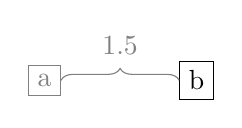
\begin{tikzpicture}
%x description="nodes with relative positioning (2)"

%x pre={
	\node[draw, gray] (a) at (0,0) {a};
%x }
%x step={
	\node[draw] (b) [right=1.5 of a] {b};
%x }

\draw [decorate, decoration={brace, amplitude=0.15cm}, gray]
	(a.east) 
	-- node [above=0.2cm] {1.5}
	(b.west);
\end{tikzpicture}

\end{document}
